\chapter{Grafteori}
\usetikzlibrary{arrows, automata}

Dette kapitel har til formål at beskrive og redegøre for forskellige grafer og de vigtigste elementer i grafteori. 
Grafer kan bruges til mange ting, blandt andet kortlægning af veje i en by, kloaksystemer og forskellige kredsløb.
En simpel graf defineres formel i definition \ref{def_simpel_graf}:


\begin{defn}
En graf $G = (V, E)$ består af $V$, et antal knuder, og E, et antal kanter hvorom der gælder at $V, E \neq \emptyset$
Hver kant har enten en eller to knuder, som den er forbundet til, som er dens endepunkter.
En kant siges at forbinde dens endepunkter. Denne konstruktion er en \it{simpel graf}.
\label{def_simpel_graf}
\end{defn}


\noindent En kant repræsenteres ved en linje mellem to knuder, og knuder repræsenteres ved et punkt. Har grafen enten et uendeligt antal knuder eller kanter, eller begge dele, er der tale om en \textit{uendelig graf}. Ellers betegnes grafen som en \textit{endelig graf}.


\begin{figure}[h]
\centering
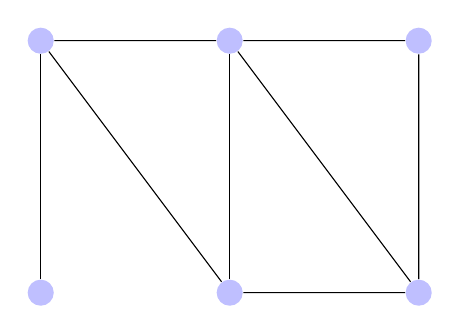
\begin{tikzpicture}
[scale=.8,auto=left,every node/.style={circle,fill=blue!25}]
  \node (n6) at (3,2) {};
  \node (n4) at (3,6) {};
  \node (n5) at (6,2) {};
  \node (n1) at (6,6) {};
  \node (n2) at (9,2) {};
  \node (n3) at (9,6) {};
  \foreach \from/\to in {n6/n4,n4/n5,n5/n1,n1/n2,n2/n5,n2/n3,n3/n1,n1/n4}
    \draw (\from) -- (\to);
\end{tikzpicture}
\caption{Et eksempel på en simpel, endelig graf} \label{simpel_graf}
\end{figure}


\noindent I figur \ref{simpel_graf} er skitseret en simpel graf med $6$ knuder og $8$ forbindende kanter. \\ 

\noindent Optræder der et uordnet punktpar ${u,v}$ i grafen, som forbindes af to eller flere kanter, kaldes grafen en \textit{multigraf}, og findes der et punkt i grafen, som via en kant forbindes med sig selv (en \textit{løkke}), er der tale om en \textit{pseudograf}. Et eksempel kan ses nedenfor for de to grafer.

\begin{figure}[!htb]
   \begin{minipage}{0.48\textwidth}
     \centering
     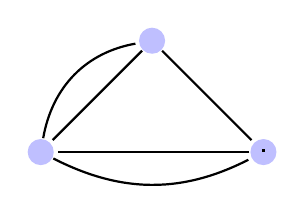
\begin{tikzpicture}[shorten >=1pt,auto,node distance=2cm,
                thick,main node/.style={circle,fill=blue!25}]

  \node[main node] (a) {};
  \node[main node] (b) [below left of=a] {};
  \node[main node] (c) [below right of=a] {};

  \path
    (a) edge node {} (b)
        edge node {} (c)
    (b) edge [bend left=35] node {} (a)
        edge [bend right=27] node {} (c)
    (c) edge [] node {} (c)
        edge node [] {} (b);

\end{tikzpicture}
     \caption{Eksempel på en multigraf}\label{Fig:Data1}
   \end{minipage}\hfill
   \begin{minipage}{0.48\textwidth}
     \centering
     \tikzset{every loop/.style={}}

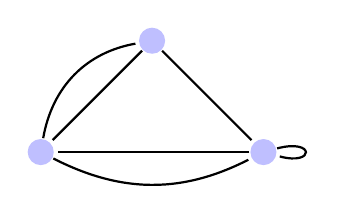
\begin{tikzpicture}[shorten >=1pt,auto,node distance=2cm,
                thick,main node/.style={circle,fill=blue!25}]

  \node[main node] (a) {};
  \node[main node] (b) [below left of=a] {};
  \node[main node] (c) [below right of=a] {};

  \path
    (a) edge node {} (b)
        edge node {} (c)
    (b) edge [bend left=35] node {} (a)
        edge [bend right=27] node {} (c)
    (c) edge [loop right] node {} (c)
        edge node [above] {} (b);
\end{tikzpicture}



     \caption{Eksempel på en pseudograf}\label{Fig:Data2}
   \end{minipage}
\end{figure}


\noindent Det kan imidlertid være nødendigt at give kanterne retning, for at indikere, hvilken retning forbindelsen mellem to punkter har. I grafer over eksempelvis trafikale netværk, kan det være nødvendigt at indikere, i hvilken retning, trafikken kører eller at angive ensrettede strækninger. Til disse formål vil en simpel graf være utilstrækkelig idet kanterne deri netop ingen bestemt retning har. Derfor anledes definition \ref{def_retn_graf} 
af en \textit{retningsbestemt graf}:

\begin{defn}
En retningsbestemt graf $G = (V, E)$ består af et antal knuder, $V$, og et antal \textit{retningsbestemte} kanter hvorom der gælder, at $V, E \neq \emptyset$.\\
En retningsbestemt kant $(u,v)$ forbinder et knudepar, så at kanten starter i $u$ og ender i $v$.
\label{def_retn_graf}
\end{defn} 

\noindent Denne definition (\ref{def_retn_graf}) tillader ydermere muligheden for, at et knudepar kan forbindes af indtil flere retningsbestemte kanter. Findes dette i grafen, kaldes den en \textit{retningsbestemt multigraf}, og denne må også indeholde løkker. I det tilfælde, at alle knudepar kun forbindes af netop én retningsbestemt kant er grafen en \textit{simpel retningsbestemt graf}.

\begin{figure}[h]
\centering
	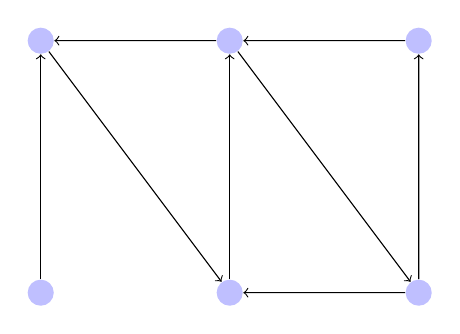
\begin{tikzpicture}
	[scale=.8,auto=left,every node/.style={circle,fill=blue!25}]
  \node (n6) at (3,2) {};
  \node (n4) at (3,6) {};
  \node (n5) at (6,2) {};
  \node (n1) at (6,6) {};
  \node (n2) at (9,2) {};
  \node (n3) at (9,6) {};
  \foreach \from/\to in {n6/n4,n4/n5,n5/n1,n1/n2,n2/n5,n2/n3,n3/n1,n1/n4}
    \draw [->] (\from) -- (\to);
	\end{tikzpicture}
\caption{Et eksempel på en retningsbestemt graf, hvor man kan se pilene definere retningen}
\end{figure}
\noindent Et simpelt retningsbestemt system er dog ikke nok i et computernetværk, som kræver at der kan forekomme flere interaktioner mellem forskellige computere. Til dette skal man bruge orienterede multigrafer.

\begin{figure}[h]
\centering
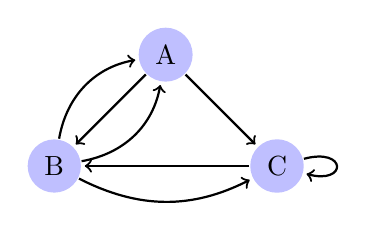
\begin{tikzpicture}[->,shorten >=1pt,auto,node distance=2cm,
                thick,main node/.style={circle,fill=blue!25}]

  \node[main node] (a) {A};
  \node[main node] (b) [below left of=a] {B};
  \node[main node] (c) [below right of=a] {C};

  \path
    (a) edge node {} (b)
        edge node {} (c)
    (b) edge [bend left=35] node {} (a)
    	    edge [bend right=35] node {} (a)
        edge [bend right=27] node {} (c)
    (c) edge [loop right] node {} (c)
        edge node [above] {} (b);
    (a) edge [bend right=30] node {} (b)
\end{tikzpicture}
\caption{Her kan man se et eksempel på en orienteret multigraf, hvor der både er adskillige kanter mellem knuderne A og B, samt er der en løkke tilstede i knudepunktet C }
\end{figure}

\noindent Nogle gange er det nødvendigt at konstruere og arbejde med computernetværker som både kan arbejde begge veje, samt ensrettet. Til dette bruger man kombineret grafer, som både indholder orienteret og ikke-orienteret kanter. Disse grafer kaldes kombinerede grafer.

\begin{figure}[!h]
\centering
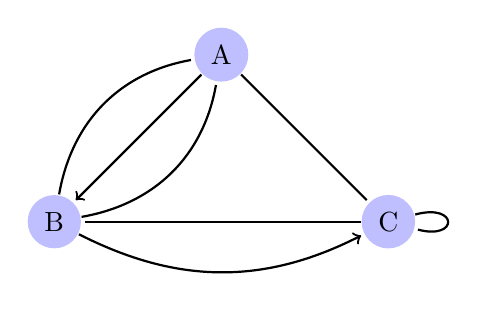
\begin{tikzpicture}[shorten >=1pt,auto,node distance=3cm,
                thick,main node/.style={circle,fill=blue!25}]

  \node[main node] (a) {A};
  \node[main node] (b) [below left of=a] {B};
  \node[main node] (c) [below right of=a] {C};

    \path [->] (a) edge node {} (b);
    \path      (a) edge node {} (c);
    \path      (b) edge [bend left=35] node {} (a);
    	\path      (b) edge [bend right=35] node {} (a);
    \path [->] (b) edge [bend right=27] node {} (c);
    \path      (c) edge [loop right] node {} (c);
    \path      (c) edge node [above] {} (b);
\end{tikzpicture}
\caption{Her kan en kombineret graf ses, hvor den både indeholder orienteret og ikke-orienteret kanter, samt indeholder den en løkke i knudepunktet C}
\end{figure}

\noindent For at kunne danne et større overblik over de forskellige grafer og deres defination og karakteristika , er tabel 5.1 konstrueret.

\begin{table}[h]
\begin{tabular}{|c|c|c|c|}
\hline 
Type & Kanter & Flerdobbelte kanter tilladt & Løkker \\ 
\hline
Simpel graf & Ikke-orienteret & Nej & Nej	 \\ 

Multigraf & Ikke-orienteret & Ja & Nej \\ 

Pseudograf & Ikke-orienteret & Ja & Ja \\ 
 
Simpel orienteret graf & Orienteret & Nej & Nej \\ 
 
Orienteret multigraf & Orienteret & Ja & Ja \\ 
 
Kombineret graf & Orienteret og ikke-orienteret & Ja & Ja \\ 
\hline 
\end{tabular}
\caption{Her kan der ses et overblik over de forskellige grafer} \label{table:graf_oversigt}
\end{table} 